\chapter{Entorno Empresarial}

En el presente capítulo se describe el entorno en el cual se desarrolló el proyecto de pasantía HxPlus Ocupacional, el cual fue realizado para la empresa Globinsoft S.A. Se presenta la historia, descripción, estructura organizacional y el cargo ocupado por el pasante dentro de la misma.

    \section{Antecedentes}
    Globinsoft S.A. posee en la actualidad su producto HxPlus el cual tiene como objetivo el almacenamiento de historias médicas de manera digital, usando tecnología web, para mantener su disponibilidad a cualquier hora del día y desde cualquier dispositivo con acceso a la web. Cuenta también con la opción de generar informes médicos, récipes y reposos médicos para uso de los farmacéutas y comodidad de los pacientes.
    
    
    \section{Misión}
    
    Brindar apoyo tecnológico al área médica en Venezuela, prestando servicios de calidad dentro del marco de lo estpulado por el Ministerio de Salud.
    
    \section{Visión}
    
    Ofrecer una plataforma integral para la gestión de consultas, historias médicas, récipes y medicamentos con alcance nacional y disponibilidad las 24 horas del día, los 7 días de la semana.
    
    \section{Estructura organizacional}
    
    Globinsoft S.A. mantiene los siguientes departamentos:
    
    \begin{enumerate}
        \item Gerencia.
        \item Recursos Humanos.
        \item Finanzas y Contabilidad.
        \item Proyectos.
    \end{enumerate}
    
    En la gerencia de proyectos se ubica el ingeniero Juán Albarrán, quien a su vez tiene el papel de tutor industrial de la pasantía descrita en el presente informe. La gerencia de proyectos se divide en cada uno de los proyectos realizados por la empresa y hasta el momento de la presente redacción, se cuenta con ``HxPlus" como proyecto en producción, al cual se le hace seguimiento, y suporte, y ``HxPlus Ocupacional" como proyecto en desarrollo. Figura \ref{estructura-org}.
    
    \begin{figure}[htbp!]
        \begin{center}
            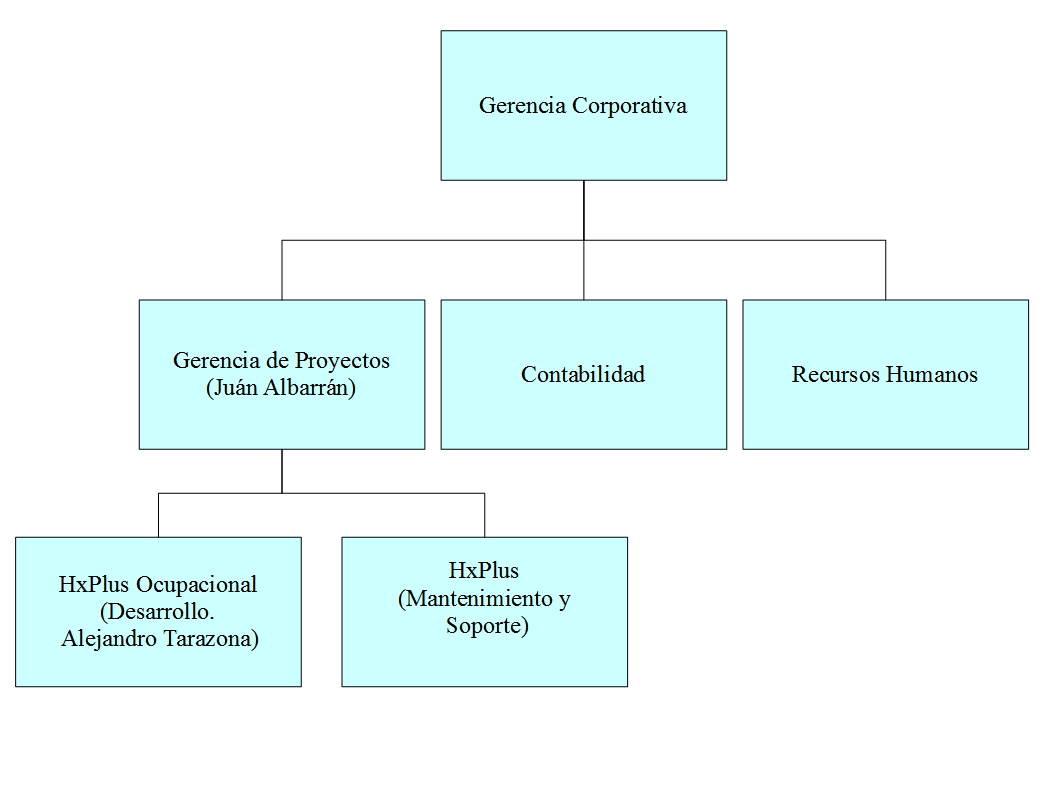
\includegraphics[width=.8\textwidth]{figures/Estructura}
        \end{center}
        \caption{Estructura Organizacional de Globinsoft}
        \label{estructura-org}
    \end{figure}

\pagebreak